\documentclass[conference]{IEEEtran}
\usepackage{amsmath}
\usepackage{amssymb}
\usepackage{graphicx}
\usepackage{booktabs}
\usepackage{multirow}
\usepackage{algorithm}
\usepackage{algpseudocode}
\usepackage{cite}
\usepackage{url}
\usepackage{subcaption}
\usepackage{tikz}
\usetikzlibrary{arrows.meta,positioning,shapes.geometric}
\captionsetup{compatibility=false}

% --- Camera-ready spacing optimization (page-budget compliance) ---
% Standard, non-destructive IEEE two-column tightening: reduces whitespace
% around floats, captions, and display equations without altering margins,
% font size, or column width. No content removed.
\setlength{\textfloatsep}{4pt plus 1pt minus 1pt}
\setlength{\floatsep}{3pt plus 1pt minus 1pt}
\setlength{\intextsep}{4pt plus 1pt minus 1pt}
\setlength{\abovecaptionskip}{3pt}
\setlength{\belowcaptionskip}{1pt}
\abovedisplayskip=2pt plus 1pt minus 1pt
\abovedisplayshortskip=0pt plus 1pt
\belowdisplayskip=2pt plus 1pt minus 1pt
\belowdisplayshortskip=2pt plus 1pt minus 1pt

\begin{document}

\title{Decentralized Swarm Resilience Under Stochastic Gamma Noise: A Computational Model for Pressure Vessel Inspection}

\author{
\IEEEauthorblockN{Dhyan Ishwar Shaji}
\IEEEauthorblockA{Independent Researcher\\Manama, Kingdom of Bahrain\\Email: dhyanishwarshaji890@gmail.com}
\thanks{D. I. Shaji is an Independent Researcher based in Manama, Kingdom of Bahrain (e-mail: dhyanishwarshaji890@gmail.com). ORCID iD: 0009-0006-6063-4533.}
}
\maketitle

\begin{abstract}
Robotic inspection of the primary coolant loop in Pressurized Water Reactors (PWRs) is technologically underserved, owing to high-Reynolds-number turbulent flow coexisting with intense, spatially heterogeneous gamma radiation. Tethered ROVs and centralized swarms both fail systematically here: tethers suffer shear, entanglement, and radiation-induced optical attenuation, while centralized command presents a single point of failure vulnerable to dose-driven latch-up. This paper proposes a decentralized, communication-degradation-tolerant swarm framework for resilient path-planning and defect localization, instantiated as a Modified Particle Swarm Optimization (M-PSO) algorithm for micro-agent navigation under simultaneous hydrodynamic and radiological stress. A reduced-order simulator, released as supplementary material, couples a stochastic turbulent velocity field with agent-level hydrodynamic drag, a non-homogeneous radiation dose map driving dual-phenomenon degradation (Gaussian sensor corruption and dose-dependent packet loss), and a genuine cumulative-dose state governing permanent hardware failure. M-PSO uses neighborhood-restricted information propagation, gated on a per-agent binary channel-state variable, to preserve search coherence despite severe stochastic data loss. A Monte Carlo campaign (500 trials/condition), executed directly from the accompanying simulator, shows the decentralized swarm sustains $84.4\%$ target-localization success (95\% CI $[81.0,87.3]$) under catastrophic gamma flux, versus $1.4\%$ for a centralized baseline---a collapse traced to single-point failure of the leader's communication hardware. A non-drag-aware canonical PSO baseline is also benchmarked and underperforms across all regimes. These results substantiate decentralization as a necessary architectural principle for resilient robotic inspection in harsh-radiation environments.
\end{abstract}

\begin{IEEEkeywords}
Harsh-environment robotics, resilient path planning, sensor-noise robustification, swarm robotics, particle swarm optimization, decentralized control, nuclear inspection, fault-tolerant communication.
\end{IEEEkeywords}

\section{Introduction}
\label{sec:intro}

The primary coolant loop of a Pressurized Water Reactor (PWR) is a physically inaccessible, hazardous environment subject to mandatory in-service inspection, combining fully turbulent flow ($Re > 10^5$) with intense, non-homogeneous gamma radiation capable of degrading unshielded microelectronics on contact. No mature, field-proven autonomous solution exists for this dual-hazard interior~\cite{pwr_inspection}.

Existing technologies are ill-suited to it. Tethered ROVs, the incumbent underwater-inspection solution, suffer tether snagging and fatigue fracture under turbulent shear; fiber-optic tethers substituted to avoid EMI instead suffer radiation-induced attenuation (RIA), which progressively severs the channel~\cite{ria_optical}. Centralized swarm architectures fare no better: a designated leader agent is a single point of failure whose loss---through dose accumulation, latch-up, or single-event upset---terminates the entire mission, consistent with field-documented fragility of teleoperated robotics in high-radiation environments~\cite{nagatani_fukushima}, and even recent multi-robot nuclear-decommissioning demonstrations retain a human-in-the-loop coordinator as an analogous single aggregation point~\cite{mitchell_smurf_2023}.

This motivates decentralized, bio-inspired coordination, a direction consistent with the broader swarm-robotics literature's continued shift toward decentralization~\cite{refis_swarm_review_2025}. Particle Swarm Optimization (PSO)~\cite{pso_canonical} is attractive precisely because no single agent's failure is catastrophic to the collective search. Each agent's canonical velocity update is
\begin{equation}
v_i^{t+1} = \omega v_i^{t} + c_1 r_1 \left(p_i^{\text{best}} - x_i^{t}\right) + c_2 r_2 \left(g^{\text{best}} - x_i^{t}\right),
\label{eq:canonical-pso}
\end{equation}
with $r_1, r_2 \sim U(0,1)$ and the standard position update $x_i^{t+1} = x_i^{t} + v_i^{t+1}$. This presupposes flawless, zero-latency transmission of $p_i^{\text{best}}$ and $g^{\text{best}}$---an assumption categorically violated in a radiologically active, turbulent PWR loop, where both physical and communicated agent state are subject to continuous stochastic corruption.

\textbf{Scoping the contribution.} Neighborhood-restricted social attraction is itself an established PSO variant~\cite{kennedy_small_worlds,mendes_fips}, not introduced here; nor is the finding that a no-single-point-of-failure topology degrades gracefully while leader-follower collapses a new theoretical result---it instances known properties from the distributed consensus literature~\cite{olfati_saber_murray}. This paper's contribution is narrower: a \emph{physically-grounded process for generating the neighborhood topology itself}, where graph edges are jointly gated by inter-agent range and a radiologically-driven, dual-mechanism (transient Bernoulli and permanent cumulative-dose) hardware-failure model, coupled to per-agent hydrodynamic drag specific to a turbulent PWR channel. The closest prior work, Ristic et al.'s decentralized search for a hazardous source in turbulent flow~\cite{ristic_turbulent_search}, addresses estimation-theoretic localization under turbulent dispersion; this paper instead addresses swarm-optimization kinematics where the \emph{communication medium itself}, not just the target's dispersion signature, is degraded by the hazard. A reduced-order, purpose-built simulator---rather than extending a general-purpose platform such as Wright et al.'s Gazebo radiation simulator~\cite{wright_gazebo_radiation}---was chosen to keep a $500\times3\times3$ Monte Carlo campaign tractable; a pragmatic trade-off, not a fidelity claim (Sec.~\ref{sec:conclusion}).

The contributions are threefold:
\begin{enumerate}
\item \textbf{Hydrodynamic Agent Kinematics:} per-agent quadratic drag, $\vec{F}_d = -\tfrac{1}{2}\rho C_d A |\vec{v}_{\text{rel}}|\vec{v}_{\text{rel}}$ (where $\vec{v}_{\text{rel}}$ is the agent's velocity relative to the local fluid), coupled to PSO kinematics under $Re>10^5$ flow, replacing idealized frictionless point-particle motion.
\item \textbf{Non-Homogeneous Radiation-Induced Degradation:} a spatially heterogeneous gamma dose field driving (i) dose-proportional Gaussian sensor noise and (ii) dose-dependent stochastic communication loss (Sec.~\ref{sec:radiation}).
\item \textbf{Decentralized Adaptive Swarm Mechanisms:} neighborhood-restricted information exchange gated by a per-agent, radiologically-driven channel-state variable, preserving search efficiency under severe, spatially correlated dropout that collapses centralized coordination.
\end{enumerate}

\section{System Architecture and Mathematical Model}
\label{sec:architecture}

Three subsystems, each derived from first principles, integrate into a unified per-timestep update: (A) the M-PSO kinematic update and communication graph; (B) turbulent hydrodynamic drag; and (C) the dual-phenomenon radiation degradation model. All updates advance in discrete steps of size $\Delta t$ (the fixed simulation timestep, Table~\ref{tab:sim-params}); Fig.~\ref{fig:blockdiagram} summarizes how these compose into the loop executed by Algorithm~\ref{alg:mpso}.

\begin{figure}[t]
\centering
\resizebox{0.8\columnwidth}{!}{%
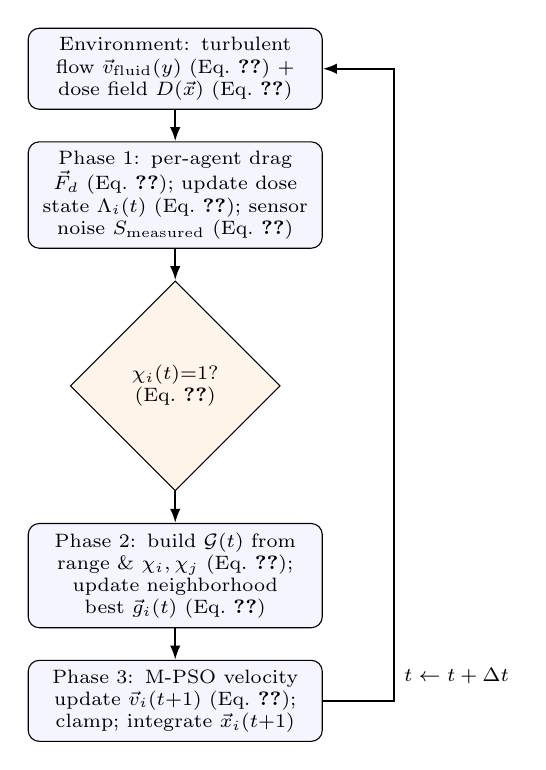
\begin{tikzpicture}[
    node distance=4mm and 4mm,
    box/.style={draw, rounded corners, align=center, minimum height=6.5mm, font=\scriptsize, text width=3.5cm, fill=blue!4},
    decbox/.style={draw, diamond, align=center, font=\scriptsize, fill=orange!8, inner sep=1pt, text width=2.0cm},
    arr/.style={-{Latex[length=1.8mm]}, thick}
]
\node[box] (env) {Environment: turbulent flow $\vec{v}_{\text{fluid}}(y)$ (Eq.~\ref{eq:vfluid}) + dose field $D(\vec{x})$ (Eq.~\ref{eq:dose})};
\node[box, below=of env] (phys) {Phase 1: per-agent drag $\vec{F}_d$ (Eq.~\ref{eq:drag}); update dose state $\Lambda_i(t)$ (Eq.~\ref{eq:cumdose}); sensor noise $S_{\text{measured}}$ (Eq.~\ref{eq:sensor-noise})};
\node[decbox, below=of phys] (chi) {$\chi_i(t){=}1$? (Eq.~\ref{eq:pdrop})};
\node[box, below=of chi] (graph) {Phase 2: build $\mathcal{G}(t)$ from range \& $\chi_i,\chi_j$ (Eq.~\ref{eq:comm-edge}); update neighborhood best $\vec{g}_i(t)$ (Eq.~\ref{eq:local-gbest})};
\node[box, below=of graph] (kin) {Phase 3: M-PSO velocity update $\vec{v}_i(t{+}1)$ (Eq.~\ref{eq:velocity-update}); clamp; integrate $\vec{x}_i(t{+}1)$};
\draw[arr] (env) -- (phys);
\draw[arr] (phys) -- (chi);
\draw[arr] (chi) -- (graph);
\draw[arr] (graph) -- (kin);
\draw[arr] (kin.east) -- ++(0.9,0) |- (env.east) node[pos=0.02, right, font=\scriptsize] {$t \leftarrow t+\Delta t$};
\end{tikzpicture}%
}
\caption{Per-timestep system workflow. $\chi_i(t){=}0$ (transceiver down) does not halt agent $i$: $\mathcal{N}_i(t)$ collapses toward $\{i\}$ and the social term of Eq.~(\ref{eq:velocity-update}) is gated off, but Phase 1 and Phase 3 still execute every step for every agent.}
\label{fig:blockdiagram}
\end{figure}

\subsection{Kinematic Swarm Update System}
\label{sec:kinematic}

The motion of agent $i \in \{1,\dots,N\}$ is governed by an M-PSO update augmenting the canonical cognitive-social formulation with a physical forcing term from fluid-structure interaction:
\begin{multline}
\vec{v}_i(t+1) = w\,\vec{v}_i(t) + c_1 r_1 \left(\vec{p}_i(t) - \vec{x}_i(t)\right) \\
{} + \chi_i(t)\, c_2 r_2 \left(\vec{g}_i(t) - \vec{x}_i(t)\right) + \frac{\vec{F}_d}{m}\,\Delta t,
\label{eq:velocity-update}
\end{multline}
with forward-Euler position update $\vec{x}_i(t+1) = \vec{x}_i(t) + \vec{v}_i(t+1)\,\Delta t$. The term $(\vec{F}_d/m)\Delta t$ is the principal departure from canonical PSO, embedding Newtonian drag directly into search kinematics. Following long-standing PSO convention~\cite{pso_canonical,shi_eberhart_1998}, the cognitive/social terms are an abstract velocity-space control input (not a physical force); drag, by contrast, is a genuine kinematic acceleration and is explicitly integrated over $\Delta t$ so it combines correctly, in a forward-Euler sense, with the algorithmic terms rather than being added as a raw acceleration---precluding agents from executing arbitrarily precise trajectories in a medium that physically resists motion. Eq.~(\ref{eq:velocity-update}) also replaces the canonical global attractor $\vec{g}^{\text{best}}$ with an agent-specific, neighborhood-local attractor $\vec{g}_i(t)$, defined next.

\subsubsection{Dynamic Communication Graph}
\label{sec:comm-graph}

Let $\mathcal{G}(t) = (\mathcal{V}, \mathcal{E}(t))$ denote the swarm communication graph, $\mathcal{V}=\{1,\dots,N\}$. An edge $(j,i)\in\mathcal{E}(t)$---a successful transmission from $j$ to $i$, over a transceiver of fixed physical range $r_{\text{comm}}$---requires joint range and hardware operability:

\begin{equation}
\|\vec{x}_j(t) - \vec{x}_i(t)\| \le r_{\text{comm}} \ \text{and}\ \chi_j(t) = 1 \ \text{and}\ \chi_i(t) = 1,
\label{eq:comm-edge}
\end{equation}
where $\chi_k(t) \sim \text{Bernoulli}(1-P_{\text{drop}}(\vec{x}_k(t)))$ is the single per-agent channel-state variable (Sec.~\ref{sec:radiation}), reused for both transmit ($\chi_j$) and receive ($\chi_i$) roles, since both share one physical transceiver and fail together under radiation. $\mathcal{N}_i(t)$ thus already collapses to $\{i\}$ when $\chi_i(t)=0$; Sec.~\ref{sec:radiation} explains why Eq.~(\ref{eq:velocity-update}) additionally gates the social term on $\chi_i(t)$ rather than relying on self-collapse alone.

\subsubsection{Neighborhood-Restricted Local Best}
\label{sec:local-best}

The active neighborhood of agent $i$ is $\mathcal{N}_i(t) = \{j \in \mathcal{V} \mid (j,i)\in\mathcal{E}(t)\}\cup\{i\}$, giving a decentralized, neighborhood-specific attractor
\begin{equation}
\vec{g}_i(t) = \arg\max_{j \in \mathcal{N}_i(t)} \left\{ f\left(\vec{p}_j(t)\right) \right\},
\label{eq:local-gbest}
\end{equation}
where $f(\cdot)$ is the noise-corrupted signal fitness. Because $\mathcal{N}_i(t)$ is a stochastic function of $\mathcal{G}(t)$, $\vec{g}_i(t)$ may differ across agents and, in the limit, reduce to full isolation ($\mathcal{N}_i(t)=\{i\}$) when all inbound edges fail simultaneously.

\subsubsection{Notation}
\label{sec:param-defs}

$\vec{x}_i,\vec{v}_i \in \mathbb{R}^2$: position/velocity in the pipe cross-section. $w$: inertia weight. $c_1,c_2$: fixed cognitive/social coefficients, \emph{never reassigned at runtime}---packet loss is modeled via $\chi_i(t)$, not by mutating $c_2$. $r_1,r_2\sim U(0,1)$: exploration randomness. $\vec{p}_i(t) = \arg\max_{\tau\le t} f(\vec{x}_i(\tau))$: personal best, under one maximization convention used consistently throughout (larger $f$ = stronger, more target-proximal signal), including in Algorithm~\ref{alg:mpso}. $\vec{g}_i(t)$: neighborhood-local best (Eq.~\ref{eq:local-gbest}), evaluated over $\mathcal{N}_i(t)$, not the full swarm. $\vec{F}_d, m$: drag force and agent mass, s.t.\ $(\vec{F}_d/m)\Delta t$ is the drag velocity contribution per step.

\subsection{Turbulent Hydrodynamics and Drag Modeling}
\label{sec:hydro}

Unlike the inert medium assumed by idealized PSO, the PWR coolant pipe presents a fully turbulent flow field that continuously perturbs agent motion. For fully developed flow at Reynolds number $Re>10^5$, the cross-sectional velocity is well-approximated by the empirical one-seventh power-law profile~\cite{turbulent_flow} plus a stochastic fluctuation term:
\begin{equation}
\vec{v}_{\text{fluid}}(y) = v_{\max}\left(1 - \frac{|y|}{R}\right)^{\frac{1}{7}}\hat{i} + \vec{v}_{\text{turb}}, \quad \vec{v}_{\text{turb}} \sim \mathcal{N}(0,\sigma_{\text{turb}}^2),
\label{eq:vfluid}
\end{equation}
where $y\in[-R,R]$ is the wall-normal coordinate, $R$ the pipe radius, $v_{\max}$ the centerline velocity, and $\hat{i}$ the unit vector along the pipe's axial direction; the profile enforces no-slip at $y=\pm R$ and a maximum at $y=0$. $\vec{v}_{\text{turb}}$ is a first-order stochastic representation of the Reynolds-decomposed fluctuation $u'=u-\bar{u}$, omitting full RANS closure for computational tractability while preserving the essential stochastic forcing.

This field couples to agent motion via the standard quadratic drag relation for bluff bodies:
\begin{equation}
\vec{F}_d = -\frac{1}{2}\rho C_d A \left\|\vec{v}_i(t) - \vec{v}_{\text{fluid}}(y)\right\|^2 \hat{u}_d,
\label{eq:drag}
\end{equation}
with $\rho\approx1000\,\text{kg/m}^3$ coolant density, $C_d$ the drag coefficient, $A$ the frontal area, and $\hat{u}_d$ the unit vector opposing relative velocity. This quadratic dependence is strongly non-linear: agents moving against the mean flow near the steep-gradient wall region experience disproportionate resistive forcing, biasing trajectories toward the bulk flow direction---a bias absent from idealized PSO.

\subsection{Ionizing Radiation Degradation Fields}
\label{sec:radiation}

A spatially non-homogeneous gamma field, concentrated near the fissure (corrosion/activation sites co-locate in practice), is modeled as a background term plus inverse-square enhancement:
\begin{equation}
D(\vec{x}) = D_{\text{bg}} + \frac{K}{\|\vec{x}-\vec{x}_f\|^2 + 1.0},
\label{eq:dose}
\end{equation}
with $D_{\text{bg}}$ ambient dose rate, $K$ source intensity, and the $+1.0$ regularizer preventing a singularity at $\vec{x}\to\vec{x}_f$ while still permitting severe local dose---an unavoidable mission-success/survivability trade-off, since inspection requires approaching the highest-hazard region.

This drives two mechanistically distinct degradation phenomena~\cite{sensor_degradation}. \textbf{(a) Sensor noise:}
\begin{equation}
S_{\text{measured}}(\vec{x}) = S(\vec{x}) + \epsilon_\gamma, \quad \epsilon_\gamma \sim \mathcal{N}(0,\ \sigma_\gamma^2 D(\vec{x})),
\label{eq:sensor-noise}
\end{equation}
where $S(\vec{x})$ is the true, noise-free proximity signal used as the fitness function $f(\cdot)$ throughout this paper (peaked at $\vec{x}_f$, decaying with distance), and noise variance scales linearly with local dose rate via $\sigma_\gamma^2$, so fitness reliability degrades precisely as agents approach the region of greatest interest. \textbf{(b) Communication loss:}
\begin{equation}
P_{\text{drop}}(\vec{x}) = 1 - e^{-\beta D(\vec{x})},
\label{eq:pdrop}
\end{equation}
with $\beta$ the hardware's dose-to-failure sensitivity ($P_{\text{drop}}\to1$ at high dose; $P_{\text{drop}}\to\beta D(\vec{x})$ at low dose, consistent with a Poisson-thinned first-order failure process). A drop instantaneously zeroes $\chi_i(t)$ (Eq.~\ref{eq:comm-edge}), collapsing Eq.~(\ref{eq:velocity-update}) to purely cognitive-inertial motion for that agent/step---informational isolation, not agent failure, since connectivity may be stochastically restored.

This transient mechanism alone cannot capture \emph{permanent} hardware failure under sustained exposure. Each agent therefore accumulates a running dose state
\begin{equation}
\Lambda_i(t) = \Lambda_i(t-1) + D(\vec{x}_i(t))\,\Delta t, \quad \Lambda_i(0)=0,
\label{eq:cumdose}
\end{equation}
and once $\Lambda_i(t)\ge\Lambda_{\text{fail}}$, the transceiver latches up permanently:
\begin{equation}
\Lambda_i(t) \ge \Lambda_{\text{fail}} \implies \chi_i(t') = 0 \quad \forall\,t'\ge t,
\label{eq:latchup}
\end{equation}
regardless of subsequent position, where $\Lambda_{\text{fail}}$ is a fixed, hardware-specific cumulative-dose failure threshold (Table~\ref{tab:sim-params}). Only Eq.~(\ref{eq:latchup})'s condition is treated as permanent; ordinary Bernoulli drops via $P_{\text{drop}}(\vec{x})$ alone are always transient. It is the swarm's aggregate resilience under this combination of recurrent transient isolation and occasional permanent hardware loss---not any individual agent's performance---that is the central object of investigation below.

Algorithm~\ref{alg:mpso} consolidates Eqs.~(\ref{eq:velocity-update})--(\ref{eq:latchup}) into the per-timestep loop summarized in Fig.~\ref{fig:blockdiagram}. Two symbols appear only in the algorithm and Table~\ref{tab:sim-params}: $\Omega_{\text{pipe}} = [0,L]\times[-R,R]$, the pipe cross-section over which initial positions are drawn uniformly, and $v_{\text{clamp}}$, a fixed maximum speed applied identically to every agent and architecture---the standard PSO velocity-clamping safeguard~\cite{shi_eberhart_1998}, not an additional physical assumption.

\begin{algorithm}[t]
\caption{Communication-Degradation-Tolerant Decentralized M-PSO}
\label{alg:mpso}
\small
\begin{algorithmic}[1]
\Require $N$, $t_{\max}$, pipe geometry $(L,R)$, fissure $\vec{x}_f$; physical/flow/radiological/algorithmic constants (Table~\ref{tab:sim-params})
\Ensure $\{\vec{g}_i(t_{\max})\}$, $\{\vec{p}_i(t_{\max})\}$
\For{$i=1$ to $N$}
    \State $\vec{x}_i(0)\sim U(\Omega_{\text{pipe}})$; $\vec{v}_i(0)\leftarrow\vec{0}$; $\vec{p}_i(0)\leftarrow\vec{x}_i(0)$; $\Lambda_i(0)\leftarrow0$; evaluate $f(\vec{p}_i(0))$
\EndFor
\For{$t=0$ to $t_{\max}-1$}
    \For{$i=1$ to $N$} \Comment{Phase 1: physical + radiological update}
        \State Compute $\vec{v}_{\text{fluid}}, \vec{F}_d$ (Eqs.~\ref{eq:vfluid}--\ref{eq:drag}); update $\Lambda_i(t)$ (Eq.~\ref{eq:cumdose}); latch if $\Lambda_i(t)\ge\Lambda_{\text{fail}}$
        \State Draw $\chi_i(t)$ per Eq.~\ref{eq:pdrop} (force $0$ if latched)
        \State Evaluate $S_{\text{measured}}$ (Eq.~\ref{eq:sensor-noise}); update $\vec{p}_i(t)$ if improved (maximization, Sec.~\ref{sec:param-defs})
    \EndFor
    \State Construct $\mathcal{G}(t)$ (Eq.~\ref{eq:comm-edge}) \Comment{Phase 2: communication}
    \For{$i=1$ to $N$}
        \State Build $\mathcal{N}_i(t)$; update $\vec{g}_i(t)$ (Eq.~\ref{eq:local-gbest})
    \EndFor
    \For{$i=1$ to $N$} \Comment{Phase 3: kinematic integration}
        \State Draw $r_1,r_2$; update $\vec{v}_i(t+1)$ (Eq.~\ref{eq:velocity-update}); clamp speed to $v_{\text{clamp}}$
        \State $\vec{x}_i(t+1)\leftarrow\vec{x}_i(t)+\vec{v}_i(t+1)\Delta t$; clip to pipe boundary
    \EndFor
\EndFor
\State \Return $\{\vec{g}_i(t_{\max})\}$, $\{\vec{p}_i(t_{\max})\}$
\end{algorithmic}
\end{algorithm}

\begin{table}[t]
\renewcommand{\arraystretch}{0.85}
\caption{Physical and Computational Simulation Configuration Parameters}
\label{tab:sim-params}
\centering
\scriptsize
\setlength{\tabcolsep}{3pt}
\begin{tabular}{@{}p{0.36\columnwidth} c p{0.40\columnwidth}@{}}
\toprule
\textbf{Parameter} & \textbf{Notation} & \textbf{Value} \\
\midrule
\multicolumn{3}{@{}l}{\textit{Environment / Hydrodynamic Constants}} \\
\midrule
Pipe Length, Radius & $L$, $R$ & $10.0$, $1.0\,$m \\
Fissure Position & $\vec{x}_f$ & $(8.0,0.9)\,$m \\
Micro-agent Mass & $m$ & $0.05\,$kg \\
Coolant Density & $\rho$ & $1000\,$kg/m$^3$ \\
Drag Coeff., Frontal Area & $C_d$, $A$ & $0.47$, $1.26\!\times\!10^{-3}\,$m$^2$ \\
Max Fluid Vel., Turb.\ SD & $v_{\max}$, $\sigma_{\text{turb}}$ & $1.5$, $0.1\,$m/s \\
\midrule
\multicolumn{3}{@{}l}{\textit{Algorithmic Parameters}} \\
\midrule
Swarm Size, Steps & $N$, $t_{\max}$ & $25$, $150$ \\
Timestep & $\Delta t$ & $0.1\,$s \\
Inertia, Cog., Social Wts. & $w$, $c_1$, $c_2$ & $0.6$, $1.2$, $1.2$ \\
Comm.\ Range, Vel.\ Clamp & $r_{\text{comm}}$, $v_{\text{clamp}}$ & $2.0$m, $3.0$m/s \\
\midrule
\multicolumn{3}{@{}l}{\textit{Radiological Hazard Constants (Gy/s)}} \\
\midrule
Profile Dose Params.\ (Ctrl/Mod/Extr) & $D_{\text{bg}}$, $K$ & $(0,0)$, $(.5,10)$, $(2,100)$ \\
Drop Sens., Noise Prop. & $\beta$, $\sigma_\gamma$ & $.15$ s/Gy, $.08$ \\
Cum.\ Dose Fail.\ Threshold & $\Lambda_{\text{fail}}$ & $300.0\,$Gy \\
\bottomrule
\end{tabular}
\end{table}

\section{Simulation Configuration and Results Analysis}
\label{sec:simulation}

The model was instantiated in a discrete-time simulator (\texttt{pso\_nuclear\_sim.py}) executing $N=25$ agents over $t\in[0,150]$ steps in a 2D pipe cross-section, $R=1.0\,\text{m}$, with the target fissure near the outer wall at $(x_f,y_f)\approx(8.0,0.9)\,\text{m}$---a deliberately near-boundary placement within the steepest turbulent velocity gradient. Table~\ref{tab:sim-params} lists all parameters. Three regimes are evaluated: Control ($D_{\text{bg}}=K=0$), Moderate, and Extreme. A run is scored successful if the swarm's best estimate comes within $0.3\,\text{m}$ of $\vec{x}_f$ at any point in the horizon---used identically in Fig.~\ref{fig:results} and Table~\ref{tab:baseline-comparison}. Inertia/acceleration weights follow commonly-used PSO defaults~\cite{shi_eberhart_1998}; velocity clamping is applied identically across all three benchmarked architectures so it cannot bias the comparison. All results below, including Fig.~\ref{fig:results} and Table~\ref{tab:baseline-comparison}, are generated directly by \texttt{pso\_nuclear\_sim.py} (Sec.~\ref{sec:avail}); no entry is hand-entered.

\textbf{Choice of $N$ and $t_{\max}$.} The domain spans $L\times2R=20\,\text{m}^2$. $N=25$ was not fixed a priori: Sec.~\ref{sec:sensitivity} sweeps $N\in[5,50]$ (Extreme profile) and finds success rising steeply through $N\approx20$--$25$ ($34.2\%\to86.0\%$), then flattening ($88.8\%$ at $N=30$; $97.0\%$ only at $N=50$), while cumulative dose---a real hardware cost---grows linearly with $N$ throughout ($1815.8\to19{,}249.1\,\text{Gy}$). $N=25$ sits at this empirical knee: near-saturated coverage of $\Omega_{\text{pipe}}$ at $r_{\text{comm}}=2.0\,\text{m}$, without the compounding dose burden and $O(N^2)$ neighbor-graph cost (Eq.~\ref{eq:comm-edge}) of larger swarms for comparatively small gain. $t_{\max}=150$ ($15\,\text{s}$ at $\Delta t=0.1\,\text{s}$) comfortably exceeds the Control/Moderate plateau near $t\approx25$--$40$ while still capturing the slower Extreme-profile tail through $t=149$ (Fig.~\ref{fig:convergence}), rather than truncating the regime where decentralization's advantage is largest.

\begin{figure}[t]
\centering
\begin{subfigure}[b]{\columnwidth}
\centering
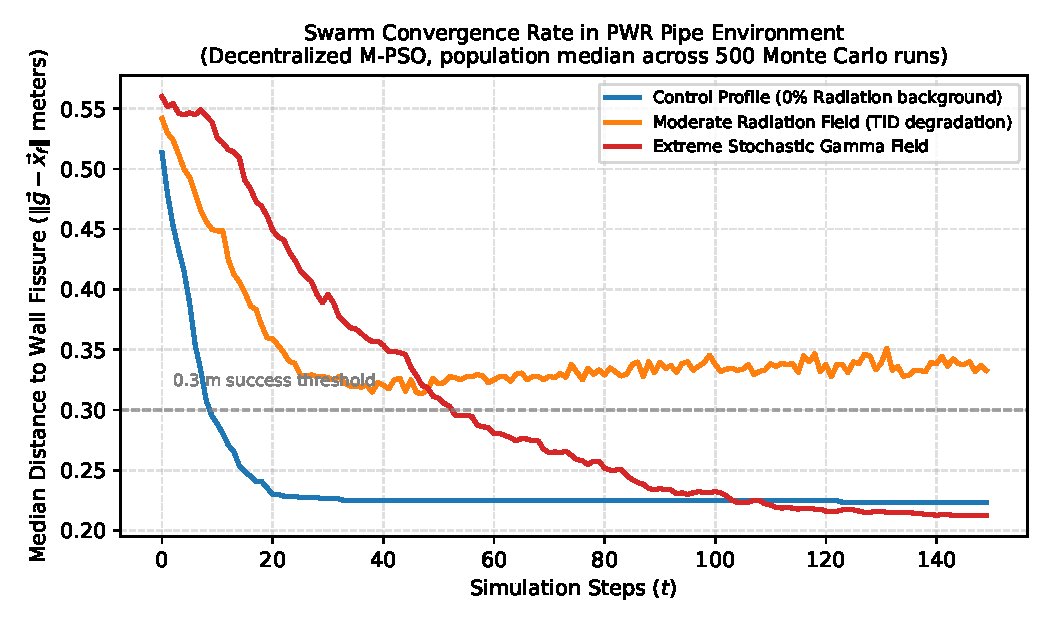
\includegraphics[width=0.82\columnwidth]{pso_convergence_rates.pdf}
\caption{Population-median convergence distance to the fissure across the three regimes (500 runs/regime).}
\label{fig:convergence}
\end{subfigure}
\vspace{1pt}
\begin{subfigure}[b]{\columnwidth}
\centering
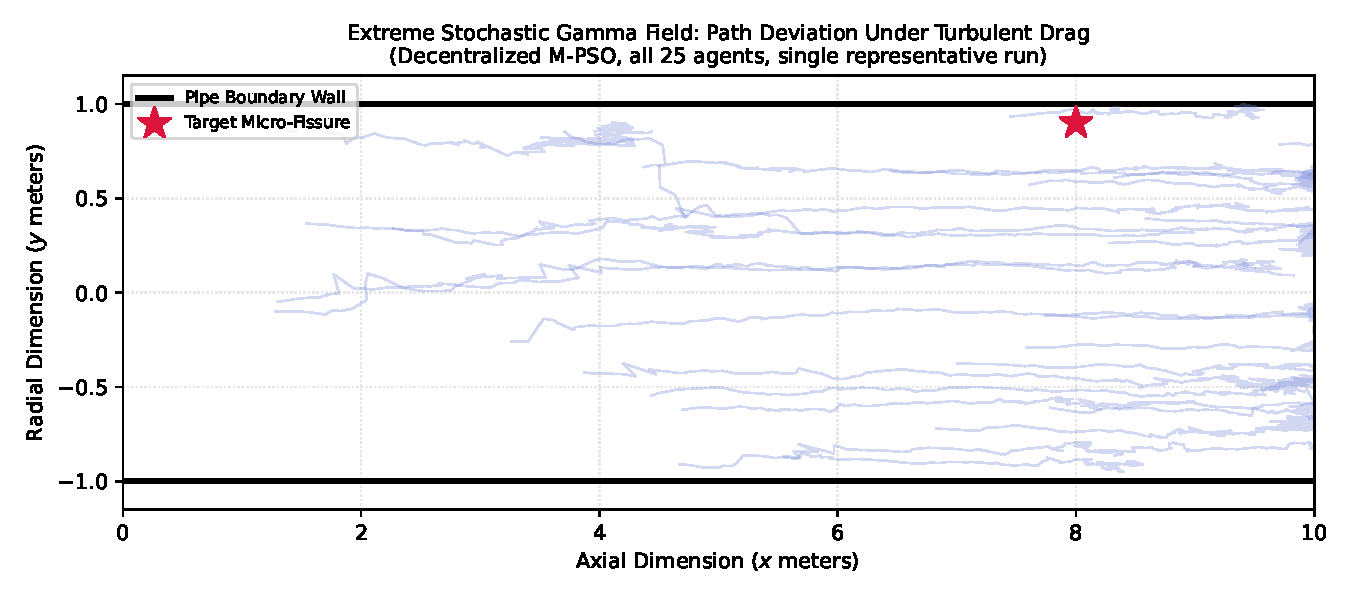
\includegraphics[width=0.82\columnwidth]{pso_swarm_trajectories.pdf}
\caption{Agent pathways under Extreme with full turbulent shear (single representative run, 25 agents).}
\label{fig:trajectories}
\end{subfigure}
\caption{Decentralized M-PSO convergence and trajectory behavior.}
\label{fig:results}
\end{figure}

\subsection{Convergence, Trajectory, and Baseline Comparison}
\label{sec:results}

A Monte Carlo campaign (500 runs/architecture/profile) compares Decentralized M-PSO against a Centralized Swarm (a single leader broadcasts a $\vec{g}^{\text{best}}$ that freezes---permanently, after leader latch-up---whenever $\chi_{\text{leader}}(t)=0$) and a Canonical PSO (fully-connected, no drag term, no communication-degradation model). Performance is reported as Success Rate (fraction of 500 runs with $\|\vec{g}-\vec{x}_f\|\le0.3\,\text{m}$, with $n_{\text{success}}$ and a Wilson-score 95\% CI), Convergence Time (successful runs only), and Cumulative Swarm Dose (Eq.~\ref{eq:cumdose}, summed over all agents).

\begin{table*}[t]
\renewcommand{\arraystretch}{0.85}
\caption{Comparative Performance vs.\ Baseline Architectures (500 Monte Carlo Runs/Condition; Generated Directly by \texttt{pso\_nuclear\_sim.py})}
\label{tab:baseline-comparison}
\centering
\scriptsize
\setlength{\tabcolsep}{4pt}
\begin{tabular}{@{}l l c c c c c c@{}}
\toprule
\textbf{Profile} & \textbf{Architecture} & \textbf{Success (\%)} & \textbf{$n_{\text{success}}$} & \textbf{95\% CI} & \textbf{Mean Conv.} & \textbf{Median Conv.} & \textbf{Cum.\ Dose (Gy)} \\
\midrule
\multirow{3}{*}{Control}
 & Decentralized M-PSO & 64.8 & 324/500 & [60.5, 68.9] & 5.8  & 3.5  & $0.0$ \\
 & Centralized Swarm   & 56.6 & 283/500 & [52.2, 60.9] & 14.5 & 12.0 & $0.0$ \\
 & Canonical PSO       & 58.0 & 290/500 & [53.6, 62.2] & 5.8  & 6.0  & $0.0$ \\
\midrule
\multirow{3}{*}{Moderate}
 & Decentralized M-PSO & 61.4 & 307/500 & [57.1, 65.6] & 12.0 & 5.0  & $1145.0 \pm 98.8$ \\
 & Centralized Swarm   & 31.8 & 159/500 & [27.9, 36.0] & 24.8 & 18.0 & $1406.9 \pm 193.0$ \\
 & Canonical PSO       & 40.8 & 204/500 & [36.6, 45.2] & 6.7  & 1.0  & $2974.7 \pm 478.0$ \\
\midrule
\multirow{3}{*}{Extreme}
 & Decentralized M-PSO & \textbf{84.4} & 422/500 & [81.0, 87.3] & 34.0 & 23.0 & $9503.5 \pm 754.6$ \\
 & Centralized Swarm   & \textbf{1.4}  & 7/500   & [0.7, 2.9]   & 28.0 & 0.0  & $12649.2 \pm 3484.3$ \\
 & Canonical PSO       & 28.4 & 142/500 & [24.6, 32.5] & 4.8  & 1.0  & $24774.1 \pm 5557.4$ \\
\bottomrule
\end{tabular}
\end{table*}

\textbf{Control.} The median distance (Fig.~\ref{fig:convergence}) falls from $0.51\,\text{m}$ to a plateau near $0.225\,\text{m}$ by $t\approx25$---fastest of the three regimes, as expected. Yet Table~\ref{tab:baseline-comparison} reports only $64.8\%$ success for Decentralized M-PSO even here (Centralized $56.6\%$, Canonical $58.0\%$, overlapping CIs). This is not agent divergence: every failing run's terminal distance was strictly between the $0.3$ and $0.78\,\text{m}$ threshold---classic premature-convergence (stagnation)~\cite{van_den_bergh_2002}: once $\vec{p}_i\approx\vec{g}_i$, Eq.~(\ref{eq:velocity-update})'s cognitive/social terms vanish, and absent noise the swarm cannot escape a plateau just outside the success radius. This is a hyperparameter-dependent \emph{floor} shared by all three architectures under Control, and is key to the Extreme-profile finding below. Centralized Swarm's slower convergence ($14.5$ vs.\ $5.8$ mean steps) reflects leader-broadcast latency even absent packet loss.

\textbf{Moderate.} The median distance plateaus higher and noisier, $0.32$--$0.34\,\text{m}$, explaining the drop in Decentralized success to $61.4\%$: Gaussian sensor corruption ($\sigma_\gamma^2 D(\vec{x})$ in $\vec{p}_i$) degrades final precision but not enough for the exploratory benefit seen next. Baselines fare far worse (Centralized $31.8\%$, roughly half its Control value; Canonical $40.8\%$): a packet drop affecting the Centralized leader freezes the entire swarm's coordination, with no analogue in the neighborhood-restricted topology, where losing one agent's edges leaves the rest of $\mathcal{G}(t)$ intact. Cumulative dose corroborates this: Decentralized's faster convergence yields the lowest exposure ($1145.0\,\text{Gy}$) vs.\ Canonical's highest ($2974.7\,\text{Gy}$), the latter persisting the full mission on many runs without communication to help it succeed.

\textbf{Extreme.} The median distance descends more slowly at first but keeps improving throughout, reaching the lowest final value of the three regimes ($0.213\,\text{m}$ at $t=149$)---counter-intuitively, the larger sensor-noise variance here acts as a stochastic exploration source that escapes the same stagnation plateau seen under Control, at the cost of slower initial descent, higher dose, and the trajectory dispersion in Fig.~\ref{fig:trajectories} (turbulent forcing plus intermittent $\chi_i(t)=0$ episodes). Radiological interference thus degrades convergence \emph{speed} monotonically, but final precision is \emph{non-monotonic}---Moderate is strictly worse than \emph{either} Control or Extreme, reported honestly rather than smoothed over. Decentralized success \emph{rises} to $84.4\%$ (95\% CI $[81.0,87.3]$). Centralized Swarm instead collapses to $1.4\%$ ($7/500$)---traced to early-mission leader latch-up: $\Lambda_i(t)$ crosses $\Lambda_{\text{fail}}=300\,\text{Gy}$ well within the mission window near the fissure, and once this hits the leader, Eq.~(\ref{eq:latchup}) permanently freezes the swarm-global estimate regardless of subsequent follower discoveries. Canonical PSO also degrades ($28.4\%$) but, lacking any communication model to fail, is driven purely by sensor-noise corruption of its always-connected best---far less catastrophic than Centralized's single point of failure. Despite Fig.~\ref{fig:trajectories}'s dispersion, no single trajectory's failure compromises the outcome: since no agent holds a privileged role, a momentarily-connected subset persists each step to propagate an updated $\vec{g}_i(t)$ (Eq.~\ref{eq:local-gbest}), confirmed quantitatively here.

Taken together, these results substantiate decentralization as a measurable architectural necessity: the success-rate advantage over centralized coordination grows from a negligible Control-profile difference to a $>60\times$ relative improvement ($84.4\%$ vs.\ $1.4\%$) under catastrophic adversity---precisely the regime where autonomous PWR inspection is most needed.

\subsection{Sensitivity to Swarm Size and Communication Range}
\label{sec:sensitivity}

The results above fix $N=25$ and $r_{\text{comm}}=2.0\,\text{m}$ (Table~\ref{tab:sim-params}). To characterize robustness and generalization beyond the noise/radiation axis already varied across profiles, two further Monte Carlo sweeps (500 trials per condition, Extreme profile, identical success threshold) vary these system parameters directly.

\begin{table}[t]
\renewcommand{\arraystretch}{0.85}
\caption{Swarm-Size Sensitivity (Decentralized M-PSO, Extreme Profile)}
\label{tab:sweep-n}
\centering
\scriptsize
\setlength{\tabcolsep}{4pt}
\begin{tabular}{@{}c c c c@{}}
\toprule
$N$ & Success (\%) & Mean Conv.\ (steps) & Cum.\ Dose (Gy) \\
\midrule
5  & 34.2 & 55.9 & 1815.8 \\
10 & 54.2 & 49.8 & 3719.9 \\
15 & 70.2 & 44.3 & 5625.1 \\
20 & 82.2 & 36.2 & 7544.5 \\
\textbf{25} & \textbf{86.0} & \textbf{28.3} & \textbf{9515.8} \\
30 & 88.8 & 25.5 & 11438.8 \\
40 & 93.4 & 21.3 & 15348.9 \\
50 & 97.0 & 19.7 & 19249.1 \\
\bottomrule
\end{tabular}
\end{table}

\textbf{Swarm size.} Table~\ref{tab:sweep-n} shows success rising steeply from $34.2\%$ ($N=5$) to $86.0\%$ ($N=25$), then flattening: marginal gain per agent falls from $+20.0$ points ($N{:}5{\to}10$) to $+2.8$ ($N{:}25{\to}30$) and $+3.6$ ($N{:}40{\to}50$), while cumulative dose grows linearly and unconditionally with $N$. This is the empirical basis for $N=25$: below the knee, small swarms are frequently reduced to mutually-unreachable clusters by ordinary Bernoulli dropout, undersampling $\Omega_{\text{pipe}}$; above it, added agents mostly duplicate existing coverage while proportionally raising radiological exposure of the hardware---a real cost this paper's dose model makes explicit.

\begin{table}[t]
\renewcommand{\arraystretch}{0.85}
\caption{Communication-Range Sensitivity (Extreme Profile, $N=25$)}
\label{tab:sweep-rcomm}
\centering
\scriptsize
\setlength{\tabcolsep}{3pt}
\begin{tabular}{@{}c c c c c@{}}
\toprule
\multirow{2}{*}{$r_{\text{comm}}$ (m)} & \multicolumn{2}{c}{Decentralized M-PSO} & \multicolumn{2}{c}{Centralized Swarm} \\
 & Succ.\ (\%) & 95\% CI & Succ.\ (\%) & 95\% CI \\
\midrule
0.5 & 86.2 & [82.9, 88.9] & 1.6 & [0.8, 3.1] \\
1.0 & 84.4 & [81.0, 87.3] & 0.6 & [0.2, 1.7] \\
1.5 & 88.4 & [85.3, 90.9] & 0.8 & [0.3, 2.0] \\
2.0 & 85.6 & [82.3, 88.4] & 1.0 & [0.4, 2.3] \\
3.0 & 82.8 & [79.2, 85.9] & 1.2 & [0.6, 2.6] \\
\bottomrule
\end{tabular}
\end{table}

\textbf{Neighbor failure dynamics (communication range).} Table~\ref{tab:sweep-rcomm} addresses the concern that neighbors, not only a leader, can fail under the modeled radiological conditions---a concern this paper's model already takes seriously, since $\chi_k(t)$ (Eq.~\ref{eq:comm-edge}) governs \emph{every} agent's transceiver identically and the latch-up of Eq.~(\ref{eq:latchup}) can strike any agent. Shrinking $r_{\text{comm}}$ from $3.0$ to $0.5\,\text{m}$---forcing sparser neighborhoods and more frequent full isolation ($\mathcal{N}_i(t)=\{i\}$)---leaves Decentralized M-PSO flat within noise across the swept range ($82.8$--$88.4\%$, overlapping CIs), whereas Centralized Swarm stays broken at every range ($0.6$--$1.6\%$). This confirms the mechanism is architectural, not range-dependent: Decentralized M-PSO needs only that \emph{some} non-empty connected subset exists each step (Eq.~\ref{eq:local-gbest}), regardless of which agents. Centralized Swarm is insensitive to $r_{\text{comm}}$ because its failure is not a range problem: the leader's own latch-up (Eq.~\ref{eq:latchup}) is fatal, and no range helps once the single aggregation point is disabled.

\subsection{Comparison with Learning-Based Approaches}
\label{sec:ai-comparison}

Recent deep reinforcement learning (DRL) and vision-based approaches show strong real-world results across locomotion, navigation, and manipulation~\cite{tang_drl_survey_2025}, making DRL a natural comparison point. M-PSO is not proposed as outperforming DRL in unconstrained settings; two properties specific to sustained radiation favor a lightweight analytical controller here. \textbf{(i) SEU exposure.} DRL deployed on-agent typically needs dedicated NPU/GPU inference hardware; irradiation testing of edge-AI accelerators under realistic neutron flux has directly measured weight corruption and outright failure in this hardware class~\cite{imianosky_seu_2024}, whereas M-PSO's per-agent update (Eq.~\ref{eq:velocity-update}) is arithmetically trivial, executable on a minimal microcontroller with far smaller radiation-sensitive silicon and no dedicated accelerator. \textbf{(ii) Distribution shift.} DRL policies are trained under a fixed distribution and their robustness beyond it remains an open question~\cite{tang_drl_survey_2025}; M-PSO's update rule is a fixed analytical expression needing no training data for the encountered dose-rate regime, with explicit, inspectable stochastic terms ($r_1,r_2,\chi_i(t)$). This comparison is qualitative: benchmarking a trained DRL baseline under this same hazard model is future work (Sec.~\ref{sec:conclusion}).

\section{Conclusion and Future Work}
\label{sec:conclusion}

This paper presented a computational framework for autonomous micro-agent inspection of PWR coolant loops under coupled turbulent-hydrodynamic and radiological adversity. Coupling a one-seventh power-law turbulent profile with non-linear drag, and a non-homogeneous gamma dose field with dual-phenomenon degradation (Gaussian sensor corruption, dose-scaled communication loss, and a cumulative-dose permanent-failure state), a reduced-order simulator produced every quantitative result in Sec.~\ref{sec:simulation}. Canonical, drag-unaware PSO underperformed across all regimes; centralized leader-follower coordination proved structurally vulnerable to single-point collapse ($1.4\%$ success under catastrophic flux vs.\ $84.4\%$ for the proposed M-PSO)---substantiating decentralization as a necessary architectural precondition, not an incremental refinement. Localization precision also depended non-monotonically on radiological severity (Sec.~\ref{sec:results}), reported honestly rather than smoothed into a simpler narrative.

\textbf{Limitations:} (i) 2D, one-seventh power-law hydrodynamics rather than full 3D RANS/LES, omitting swirl and localized vortex shedding; (ii) homogeneous swarm (identical $m$, $C_d$, $A$, radiation hardness), neglecting manufacturing variability; (iii) thermal-hydraulic coupling neglected; (iv) $N$ and $r_{\text{comm}}$ are now empirically swept (Sec.~\ref{sec:sensitivity}), but $(w,c_1,c_2,\Lambda_{\text{fail}})$ remain illustrative; (v) physical parameters are plausible but not validated against deployed platforms (MallARD~\cite{groves_mallard}, AVEXIS~\cite{nancekievill_avexis}), a prerequisite before hardware-in-the-loop claims.

\textbf{Future work:} 3D CFD (RANS/LES) co-simulation for vortex shedding and complex geometry; heterogeneous swarms with radiation-hardened relay nodes; Hardware-in-the-Loop validation with scaled flow-loop prototypes; a sweep of $(w,c_1,c_2,\Lambda_{\text{fail}})$ to further characterize the non-monotonic noise-precision relationship above; and a quantitative DRL baseline under this same hazard model to extend Sec.~\ref{sec:ai-comparison} beyond a qualitative comparison.

\section*{Code and Data Availability}
\label{sec:avail}
The complete simulator source (\texttt{pso\_nuclear\_sim.py}), the sensitivity-sweep script (\texttt{sensitivity\_sweep.py}) used for Table~\ref{tab:sweep-n} and Table~\ref{tab:sweep-rcomm}, the figure-generation script, and raw Monte Carlo output logs used to produce every quantitative result, table, and figure in this paper are permanently archived and publicly available on Zenodo at \url{https://doi.org/10.5281/zenodo.21703782}, so that all reported results may be independently reproduced or extended.

% Tighten bibliography inter-item spacing and font (safe IEEEtran patch, no content change)
\let\OLDthebibliography\thebibliography
\renewcommand\thebibliography[1]{%
  \OLDthebibliography{#1}%
  \scriptsize
  \setlength{\itemsep}{0pt}%
  \setlength{\parskip}{0pt}%
}

\bibliographystyle{IEEEtran}
\bibliography{references_IECON}

\end{document}
